\documentclass[a4paper, 12pt]{article}
 
\usepackage[utf8]{inputenc}
\usepackage{graphicx}
\usepackage[french]{babel}
\usepackage[T1]{fontenc}
\usepackage{lmodern}
\usepackage[top=2cm, bottom=1.5cm, left=1.5cm, right=1.5cm]{geometry}
 
\begin{document}
 
\title{Programming Assignment 1 \\ Machine Learning for Computer Vision}
\author{Mathurin \textsc{Massias} \and Clément \textsc{Nicolle}}
\date{\today} 
 
\maketitle

\section{Linear versus logistic regression}

We implemented the sigmoid function and the gradient and hessian calculus. Then, at each step, we calculate w thanks to the Newton-Raphson's method. On test data, the linear regression results in 112 errors, versus 64 only for the logistic regression.

The results are shown here :

\begin{figure}[!htbp]
\centering
\noindent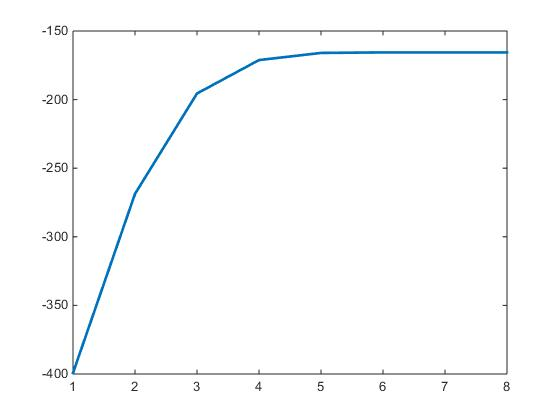
\includegraphics[scale=0.4]{images/ass1-img1.jpg}
\noindent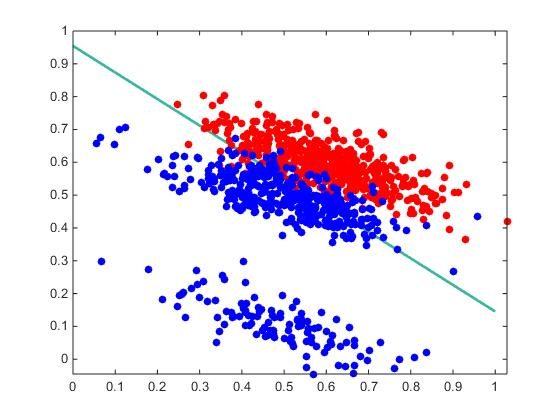
\includegraphics[scale=0.4]{images/ass1-img2.jpg}
\noindent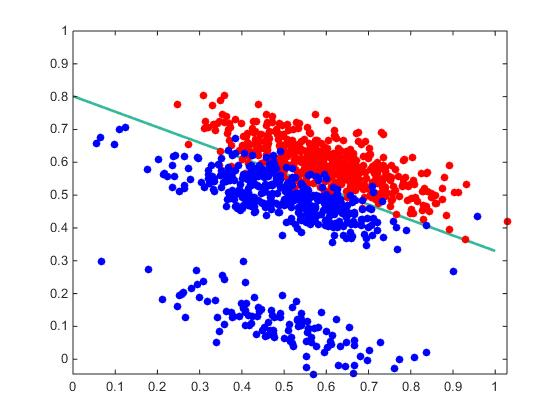
\includegraphics[scale=0.4]{images/ass1-img3.jpg}
\caption{Left: C(w) as a function Newton-Raphson iteration; middle: decision boundary for linear regression (already implemented); right: decision boundary for logistic regression}
\end{figure}

\section{Logistic Regression and Regularization}

We added a parameter "lambda" in the functions "gradient.m" and "hessian.m" to take into account the regularization term. 20 values of lambda are tested,  and 10 cross-validations are made for each lambda.

We find an optimal lambda of 5,5. Here are the averaged losses for each lambda, and the decision boundary obtained on the test set :

\begin{figure}[!htbp]
\centering
\noindent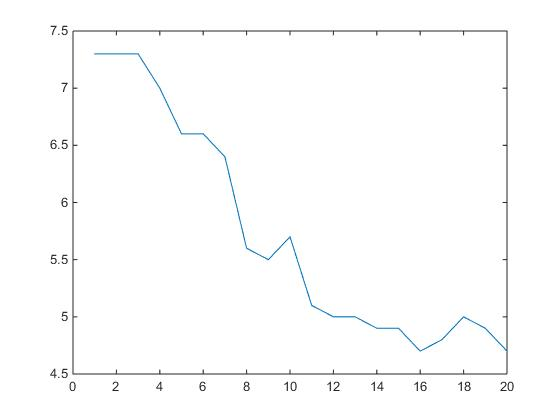
\includegraphics[scale=0.4]{images/ass1-img4.jpg}
\noindent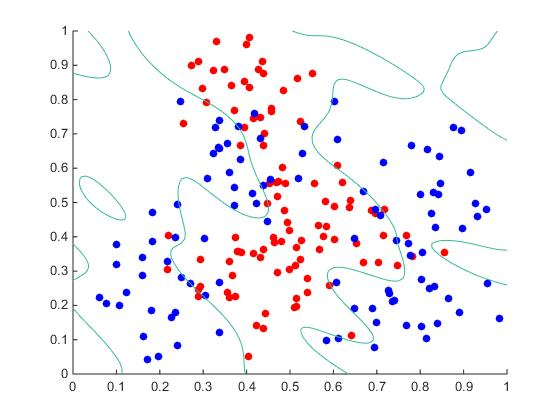
\includegraphics[scale=0.4]{images/ass1-img5.jpg}
\caption{Figure 2: Cross-validation error as a function of $\lambda$ and decision boundary for $\lambda *$}
\end{figure}

On test set, we find 49 errors.

\end{document}
